\part{Introduction}

\section {Introduction}

% task 
% traditional method
% current method
% lack of current method
% main update of your method
% additional output

3D Display System aims to proide immersive and interactive experiences of virtual scenarios base on human vision illusions. Since the concept of metaverse is introduced by Facebook, 3D display technology is attracting more and more attetion from both academic and industrial field.

While earlier 3D display base on binocular vision by allying two images as binocular disparity, the traditional 3D display system usually requires professional photographic capture devices and specialized glasses, which limits the accessibility and convenience of the system. Recent years naked-eye display systems based on horizontal parallax coms into public view. L-shaped monitor on Taiguli Chengdu(Figure 1a) is a typical example of horizontal parallax illusion applications, since the shape provide additional depth illusion.\cite{Wang2024} Althought the L-shaped display system excuse users from wearing heavy glasses, the expensive price and fixed position of the viewer still limit its accessibility and convenience.

\begin{figure}[htb]
    \centering
    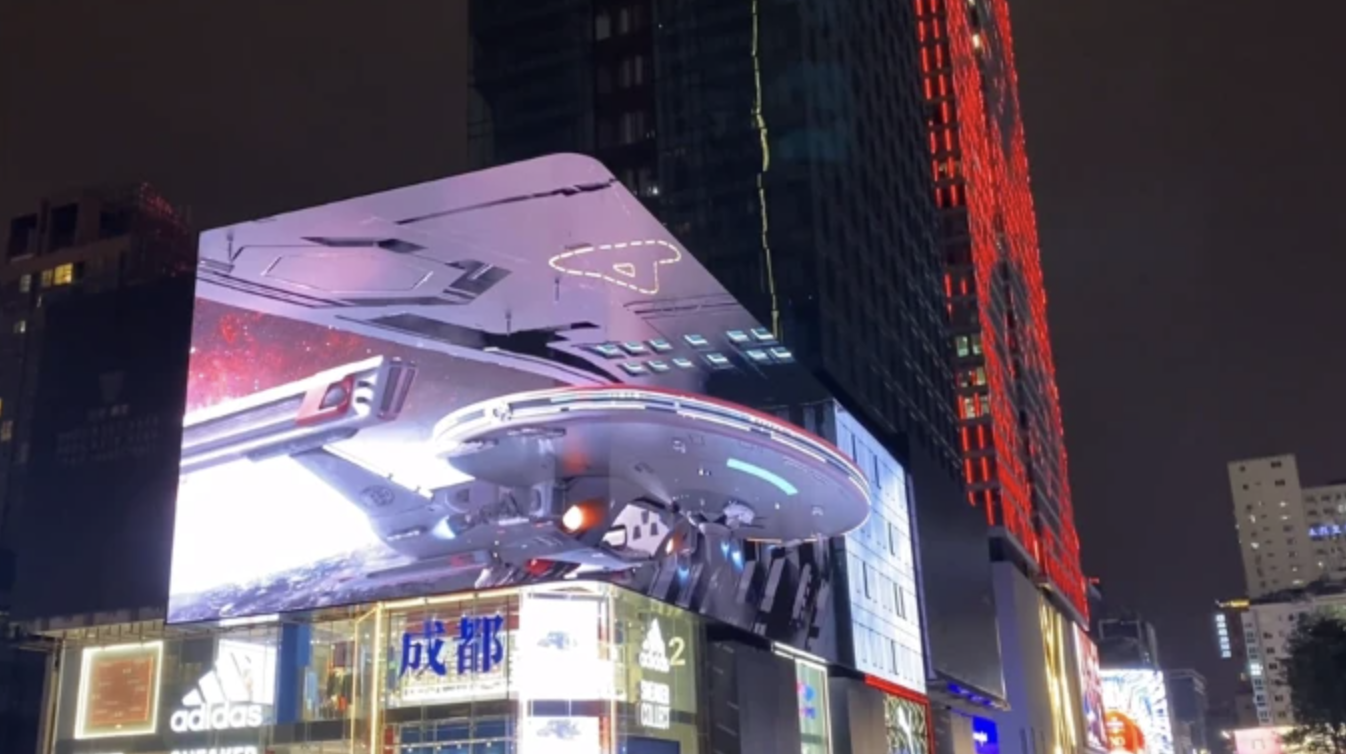
\includegraphics[width=0.7\textwidth]{figures/L-shaped.png}
    \caption{L-shaped Display Monitor}\label{F:test-a}
\end{figure}

To tackle these problems, another motion parallax based light-weight solution is proposed\cite{ALLISON20031879}. Wang\cite{Wang_2018} introduce a 3D display system based on Kinect SDK, and Peder. 2019 \cite{TheParallaxView} developed an IOS application based on iPhoneX's TrueDepth camera(Figure 1b). These two systems both use the combination of head-track and off-axis perspective projection, provided a customer-oriented 3D display system. Compare with L-shaped solutions, motion-based 3D display system is more flexible and cheaper, since it only requires a camera and a display device.

\begin{figure}[htb]
    \centering
    \includegraphics[width=0.6\textwidth]{example-image-a}
    \caption{Horizontal Parallax}\label{F:test-a}
\end{figure}

However, the head-track part in these two systems is essentially using SDK procided by hardware manufacturers(Kinect in Wang's work, and iPhone in Pader's work), which suffers from hardward limitations. Although depth measurement devices exactly provides a more convenience and stable solution, the flexibility and expensibility cannot reach requirements. Consider a general head-track task which need to inference human head's position, given a specific usage scenary, a head-track task requirement usually need to cover difference specific conditions. For example, laptop deployments without an external depth camera or laser radar. Also, SDK-based traking solutions is not flexible enough to handle possible bugs and errors, since the source code is not open to the public, makes it's harder to be mentained by single developer. In additional, SDK-based solution can only be deployed as assemblyies or on specific devices: the former needs extra cost for expensive professional devices, and the latter limits the system's application for different users, which introduce extra cost and limit naked 3d systems' further application.

\begin{figure}[htb]
    \centering
    \includegraphics[width=0.5\textwidth]{example-image-a}
    \caption{Head Track Working Flow. }\label{F:test-a}
\end{figure}

This work proposed a new head-track solution based on monocular distance measurement and off-axis projection, privide a cheaper and more flexible solution for 3D display system. As shown in figure 2, this work can inference human head's position with a single camera with the support of face landmark detection algotithm and researches of perspective-n-point(PnP) problem, without surpports of depth measurement hardwares. The main update of this work is the combination of face landmark detection and ePnP algorithm\cite{EPnP_2009}, which provide a more flexible and cheaper solution for 3D display system. 

\begin{figure}[htb]
    \centering
    \includegraphics[width=0.5\textwidth]{example-image-a}
    \caption{Image correction}\label{F:test-a}
\end{figure}

Beside monocular head-tracking, display optimization is also considered as an important of vision illusions. Since most of motion parallax based 3d systems only consider standard display monitors, we proposed a noval correction algorithm for curved displays. By accepting result from head-traking algorithms, correction algorithm can adjust displayed frames to fit the view angle of users, which is more appropriate for curved displays which is more and more popular in recent years.

The contributions of this work include:

\begin{itemize}
    \item A new head-track system based on monocular distaance measurement, which provide a cheaper and more flexible solution for 3D display system compared with depth-camera based methods.
    \item A correction algorithm for curved displays, which is more appropriate for curved displays which is more and more popular in recent years.
\end{itemize}

In conclusion, this work provides a new head-track system based on monocular distaance measurement, which is more flexible and cheaper than traditional depth-camera based methods. Conbined with off-axis perspective projection and the correction algorithm for curved displays, this work provides a more flexible and cheaper solution for 3D display system.


\section {Related Work}

\subsection {Motion Parallax}

Motion parallax is a visual illusion that occurs when objects at different distances move across the observer's field of view. This phenomenon is a key depth cue in human vision, enabling the perception of depth and distance in the absence of stereoscopic vision. Principles of motion parallax can provide depth information to human brain's neural is the comparation of motion speed of different objects in the same view. e.g., when a person moves his head, objects closer to the observer appear to move faster than objects further away, providing a sense of depth and distance. Hanes et al.(2008) explain the mathemetical details of motion parallax, providing geometry and experimental evidence of it\cite{Hanes2008}, shown as Fig.3.

\begin{figure}[htb]
    \centering
    \includegraphics[width=0.5\textwidth]{example-image-a}
    \caption{Motion parralax reminder: $d\theta / dt$ is a good cue for motion derectory, while $w(D, \theta)$ is velocity's\cite{Hanes2008}}\label{F:test-a}
\end{figure}

This effect is widely used in 3D display systems: Lee et al. (2019) designed a head-traking system based on Nintendo Wii remote, constructed a depth illusion with the application of motion parallax\cite{Lee}. Apple's IOS7 also introduced a light motion parallax effect. By move applications' icons lightly when users move their phone, Apple provides a more immersive and interactive experience for users.\cite{Apple2014}.
\subsection{Face  Landmark Detection}
From early techniques, face landmark is mainly implemented by statistical and simple machine learning methods. The \textbf{Active Shape Model (ASM)}, \textbf{Active Appearance Model (AAM)}, and \textbf{Constrained Local Model (CLM)} \cite{WANG201850} \cite{Khabarlak_2022} are foundational methods that employ statistical models to fit a deformable face mesh, optimized for controlled environments but underperforming in in-the-wild scenarios. Subsequent advancements, such as \textbf{Ensemble of Regression Trees (ERT)} \cite{Kazemi_2014_CVPR} employed by \textbf{dlib}, improved accuracy by using a cascade based on gradient boosting, making it highly efficient for real-time applications despite its limitations with pose variations.

\begin{figure}[htb]
    \centering
    \includegraphics[width=0.5\textwidth]{example-image-a}
    \caption{cascade based gradient boosting }\label{F:test-a}
\end{figure}

The evolution towards neural network-based approaches has introduced a diverse array of backbones, enhancing the detection capabilities under unconstrained conditions. Techniques such as the \textbf{Hourglass} \cite{Newell_2016_ECCV} and \textbf{HRNet} \cite{Sun_2019_CVPR} architectures leverage heatmap-based methods to improve landmark localization accuracy by predicting probabilistic heatmaps for each landmark . These methods are robust against pose variations and occlusions, crucial for applications requiring high fidelity in dynamic environments.
\textbf{Style Aggregated Network (SAN)}\cite{Dong_2018_CVPR} employs ResNet-152 \cite{He_2016_CVPR} to handle variability in image styles by stabilizing landmark detection across different photographic conditions, illustrating the importance of adaptive models in diverse real-world applications.

YOLO-series\cite{Redmon_2016_CVPR} are also considered as a efficient method in face landmark detection. As a one-stage object detection model, YOLO detect objects' position and classes by directly inference features extract by CNN model. Base on YOLO, Qi et al. (2022) developed \textbf{YOLO5Face}\cite{Qi2022YOLO5Face}, a face detector built upon the YOLOv5 object detection framework. The model incorporates modifications such as a landmark regression head and various optimizations for processing both large and small faces effectively. YOLO5Face is designed to provide robust face detection capabilities across different model sizes, catering to various application requirements from high-performance setups to real-time detection on mobile or embedded devices. The detector achieves state-of-the-art performance on the WiderFace dataset, demonstrating its efficiency and accuracy in diverse conditions. In following two years, YOLOv7-face\cite{YOLOv7Face} and YOLOv8-face\cite{YOLOv8Face} is developed, which further improve the performance of face detection and landmark detection.

\begin{figure}[htb]
    \centering
    \includegraphics[width=0.6\textwidth]{example-image-a}
    \caption{YOLOv1 structure}\label{F:test-a}
\end{figure}

In 2023, Wu et developed \textbf{YuNet}\cite{Wu_2023}, an advanced face detection model specifically engineered for edge computing devices, which emphasizes minimal model size and maximized computational efficiency. The architecture of YuNet incorporates a streamlined feature extraction backbone and a simplified pyramid feature fusion technique, tailored to meet the stringent performance requirements of mobile and embedded systems with limited processing capabilities. This model is distinguished by its ability to deliver high-speed performance with an exceptionally low parameter count, making it particularly well-suited for real-time applications where both speed and accuracy are critical, yet resources are constrained.


\subsection{Target Tracking}
During these decades, target traking problem has gains lots of attetion in academic and industrial firld due to the universality of application. With sensor information stream input, tracking algorithms estimate target's motion state, applicated them in next-timestamp's pose estimation. Target tracking algorithms can mainly be divided into three categories: \textbf{Batch Processing}, \textbf{Recursive} and \textbf{Optimization-Based}\cite{KumarMondal2021}. Batch Processing methods observe one time period operate one specific time period to estimate target's motion state, with common algorithms like MLE, PLS, GA and sequencial networks. A typical problem of Batch Processing latency issue and data requirement, since batch processing need to wait for all data to be collected before processing.\cite{KumarMondal2021}. 

Recursive-based methods, typically Sequential Bayesian filter, performance better in real-time tracking and unbiased estimates\cite{KumarMondal2021}. One powerfule variant of Sequential Bayesian filter is Kalman Filter, proposed by Rudolf E. Kálmán in 1960\cite{Kalman1960}, designed to estimate target's motion state with noisy sensor information. Kalman Filter is widely used in target tracking, pose estimation, and sensor fusion.
\begin{figure}[htb]
    \centering
    \includegraphics[width=0.6\textwidth]{example-image-a}
    \caption{Kalman Filter Working Flow}\label{F:test-a}
\end{figure}

Another category of target tracking is Optimization-Based methods, developed on the basis of loss functions of tracking methods.\cite{KumarMondal2021}. Optimization-Based methods are more flexible and can be applied in various tracking scenarios, with common algorithms like Particle Filter, Mean Shift, and Deep Learning-based methods. However, since loss-fucntions' optimization introduce extra complexity, Optimization-Based methods are usually more computational expensive than Recursive-based methods.

\nocite{Khabarlak_2022}



